% Apresentação parcial condensada (5 a 7 minutos) — IND2616: Séries Temporais
% Compile duas vezes com pdflatex para atualizar a numeração de páginas.
\documentclass[10pt,aspectratio=169]{beamer}

\usepackage[utf8]{inputenc}
\usepackage[T1]{fontenc}
\usepackage[brazil]{babel}
\usepackage{graphicx}
\usepackage{amsmath}
\usepackage{xcolor}

\definecolor{pucnavy}{RGB}{7,27,51}
\definecolor{pucblue}{RGB}{18,100,163}
\definecolor{puccyan}{RGB}{50,180,200}
\definecolor{pucorange}{RGB}{246,160,65}
\definecolor{pucgray}{RGB}{96,112,138}

\setbeamertemplate{navigation symbols}{}
\setbeamercolor{structure}{fg=pucblue}
\setbeamercolor{frametitle}{fg=pucnavy,bg=white}
\setbeamerfont{frametitle}{series=\bfseries,size=\Large}
\setbeamercolor{normal text}{fg=pucnavy,bg=white}
\setbeamercolor{block title}{fg=white,bg=pucblue}
\setbeamercolor{block body}{fg=pucnavy,bg=blue!4}
\setbeamertemplate{itemize item}{\color{pucorange}$\blacktriangleright$}
\setbeamertemplate{footline}{%
  \leavevmode\hbox{%
  \begin{beamercolorbox}[wd=.78\paperwidth,ht=2.8ex,dp=1.2ex,leftskip=1.5em]{author in head/foot}%
    \color{pucgray}\scriptsize IND2616: Séries Temporais \quad | \quad PUC-Rio
  \end{beamercolorbox}%
  \begin{beamercolorbox}[wd=.22\paperwidth,ht=2.8ex,dp=1.2ex,rightskip=1.5em plus1fil]{date in head/foot}%
    \color{pucgray}\scriptsize\insertframenumber/\inserttotalframenumber
  \end{beamercolorbox}}%
}

\graphicspath{{figuras/}}
\title{Previsão de internações por VSR em crianças menores de dois anos}
\subtitle{Apresentação parcial \quad | \quad 5 a 7 minutos}
\author{Thiago Paes \and Joan Souza \and Matheus Accioly \and Isabelle Gagno}
\institute{Mestrado PUC-Rio \quad | \quad IND2616: Séries Temporais \quad | \quad Prof. Fernando Cyrino}
\date{Outubro de 2026}

\begin{document}

\begin{frame}[plain]
  \colorbox{pucnavy}{%
    \parbox[c][\paperheight][c]{\paperwidth}{%
      \vspace{.7cm}
      \hspace{1.2cm}\textcolor{puccyan}{\Large\textbf{IND2616: Séries Temporais}}\\[1.0cm]
      \hspace{1.2cm}\parbox{.78\paperwidth}{\color{white}\fontsize{30}{35}\selectfont\bfseries Previsão de internações por VSR em crianças menores de dois anos}\\[.5cm]
      \hspace{1.2cm}\parbox{.72\paperwidth}{\color{white}\large Uma análise temporal de hospitalizações por SRAG associadas ao vírus sincicial respiratório no Brasil.}\\[1cm]
      \hspace{1.2cm}\color{white}\normalsize Thiago Paes \quad Joan Souza \quad Matheus Accioly \quad Isabelle Gagno\\[.25cm]
      \hspace{1.2cm}\color{white}\normalsize Mestrado PUC-Rio \quad | \quad Professor Fernando Cyrino
      \vfill
    }%
  }
\end{frame}

\begin{frame}{Problema e dados do estudo}
  \begin{columns}[T,onlytextwidth]
    \begin{column}{.54\textwidth}
      \large Como antecipar a quantidade semanal de internações por VSR antes da chegada de uma onda sazonal?\par\vspace{.35cm}
      \begin{itemize}
        \item O foco é previsão para apoiar o planejamento de leitos pediátricos, equipes e insumos.
        \item A unidade de análise é a contagem semanal de internações confirmadas por VSR.
        \item O painel contém UF, regiões e Brasil.
      \end{itemize}
    \end{column}
    \begin{column}{.42\textwidth}
      \textcolor{pucblue}{\Large\textbf{4.679.012}}\\[-.1cm]
      \small registros brutos de SRAG, SIVEP-Gripe, 2019--2026.\\[.38cm]
      \textcolor{pucblue}{\Large\textbf{158.358}}\\[-.1cm]
      \small notificações únicas no recorte final.\\[.38cm]
      \small \textbf{Recorte:} SRAG hospitalizada, criança menor de dois anos, VSR confirmado por PCR ou antígeno, UF válida e início dos sintomas disponível.
    \end{column}
  \end{columns}
\end{frame}

\begin{frame}{Tratamento e confiabilidade da série}
  \begin{columns}[T,onlytextwidth]
    \begin{column}{.31\textwidth}
      \textcolor{pucblue}{\textbf{Recorte e auditoria}}\\[.12cm]
      \small Verificamos arquivos, campos, datas, códigos laboratoriais e unidade geográfica antes de agregar os registros.
    \end{column}
    \begin{column}{.31\textwidth}
      \textcolor{pucblue}{\textbf{Duplicidades}}\\[.12cm]
      \small Dois pares com o mesmo identificador foram auditados e resolvidos por regra temporal documentada.
    \end{column}
    \begin{column}{.31\textwidth}
      \textcolor{pucblue}{\textbf{Semanas maduras}}\\[.12cm]
      \small Usamos 13 semanas de maturação para reduzir sub-registro temporário por atraso de notificação ou confirmação.
    \end{column}
  \end{columns}
  \vspace{.45cm}
  \begin{block}{Base usada nas análises}
    Registros individuais foram agregados em semanas epidemiológicas. O histórico analítico contém 395 semanas maduras; as 12 semanas mais recentes não são tratadas como verdade final da avaliação.
  \end{block}
\end{frame}

\begin{frame}{Padrões exploratórios: sazonalidade e diferenças geográficas}
  \begin{columns}[T,onlytextwidth]
    \begin{column}{.56\textwidth}
      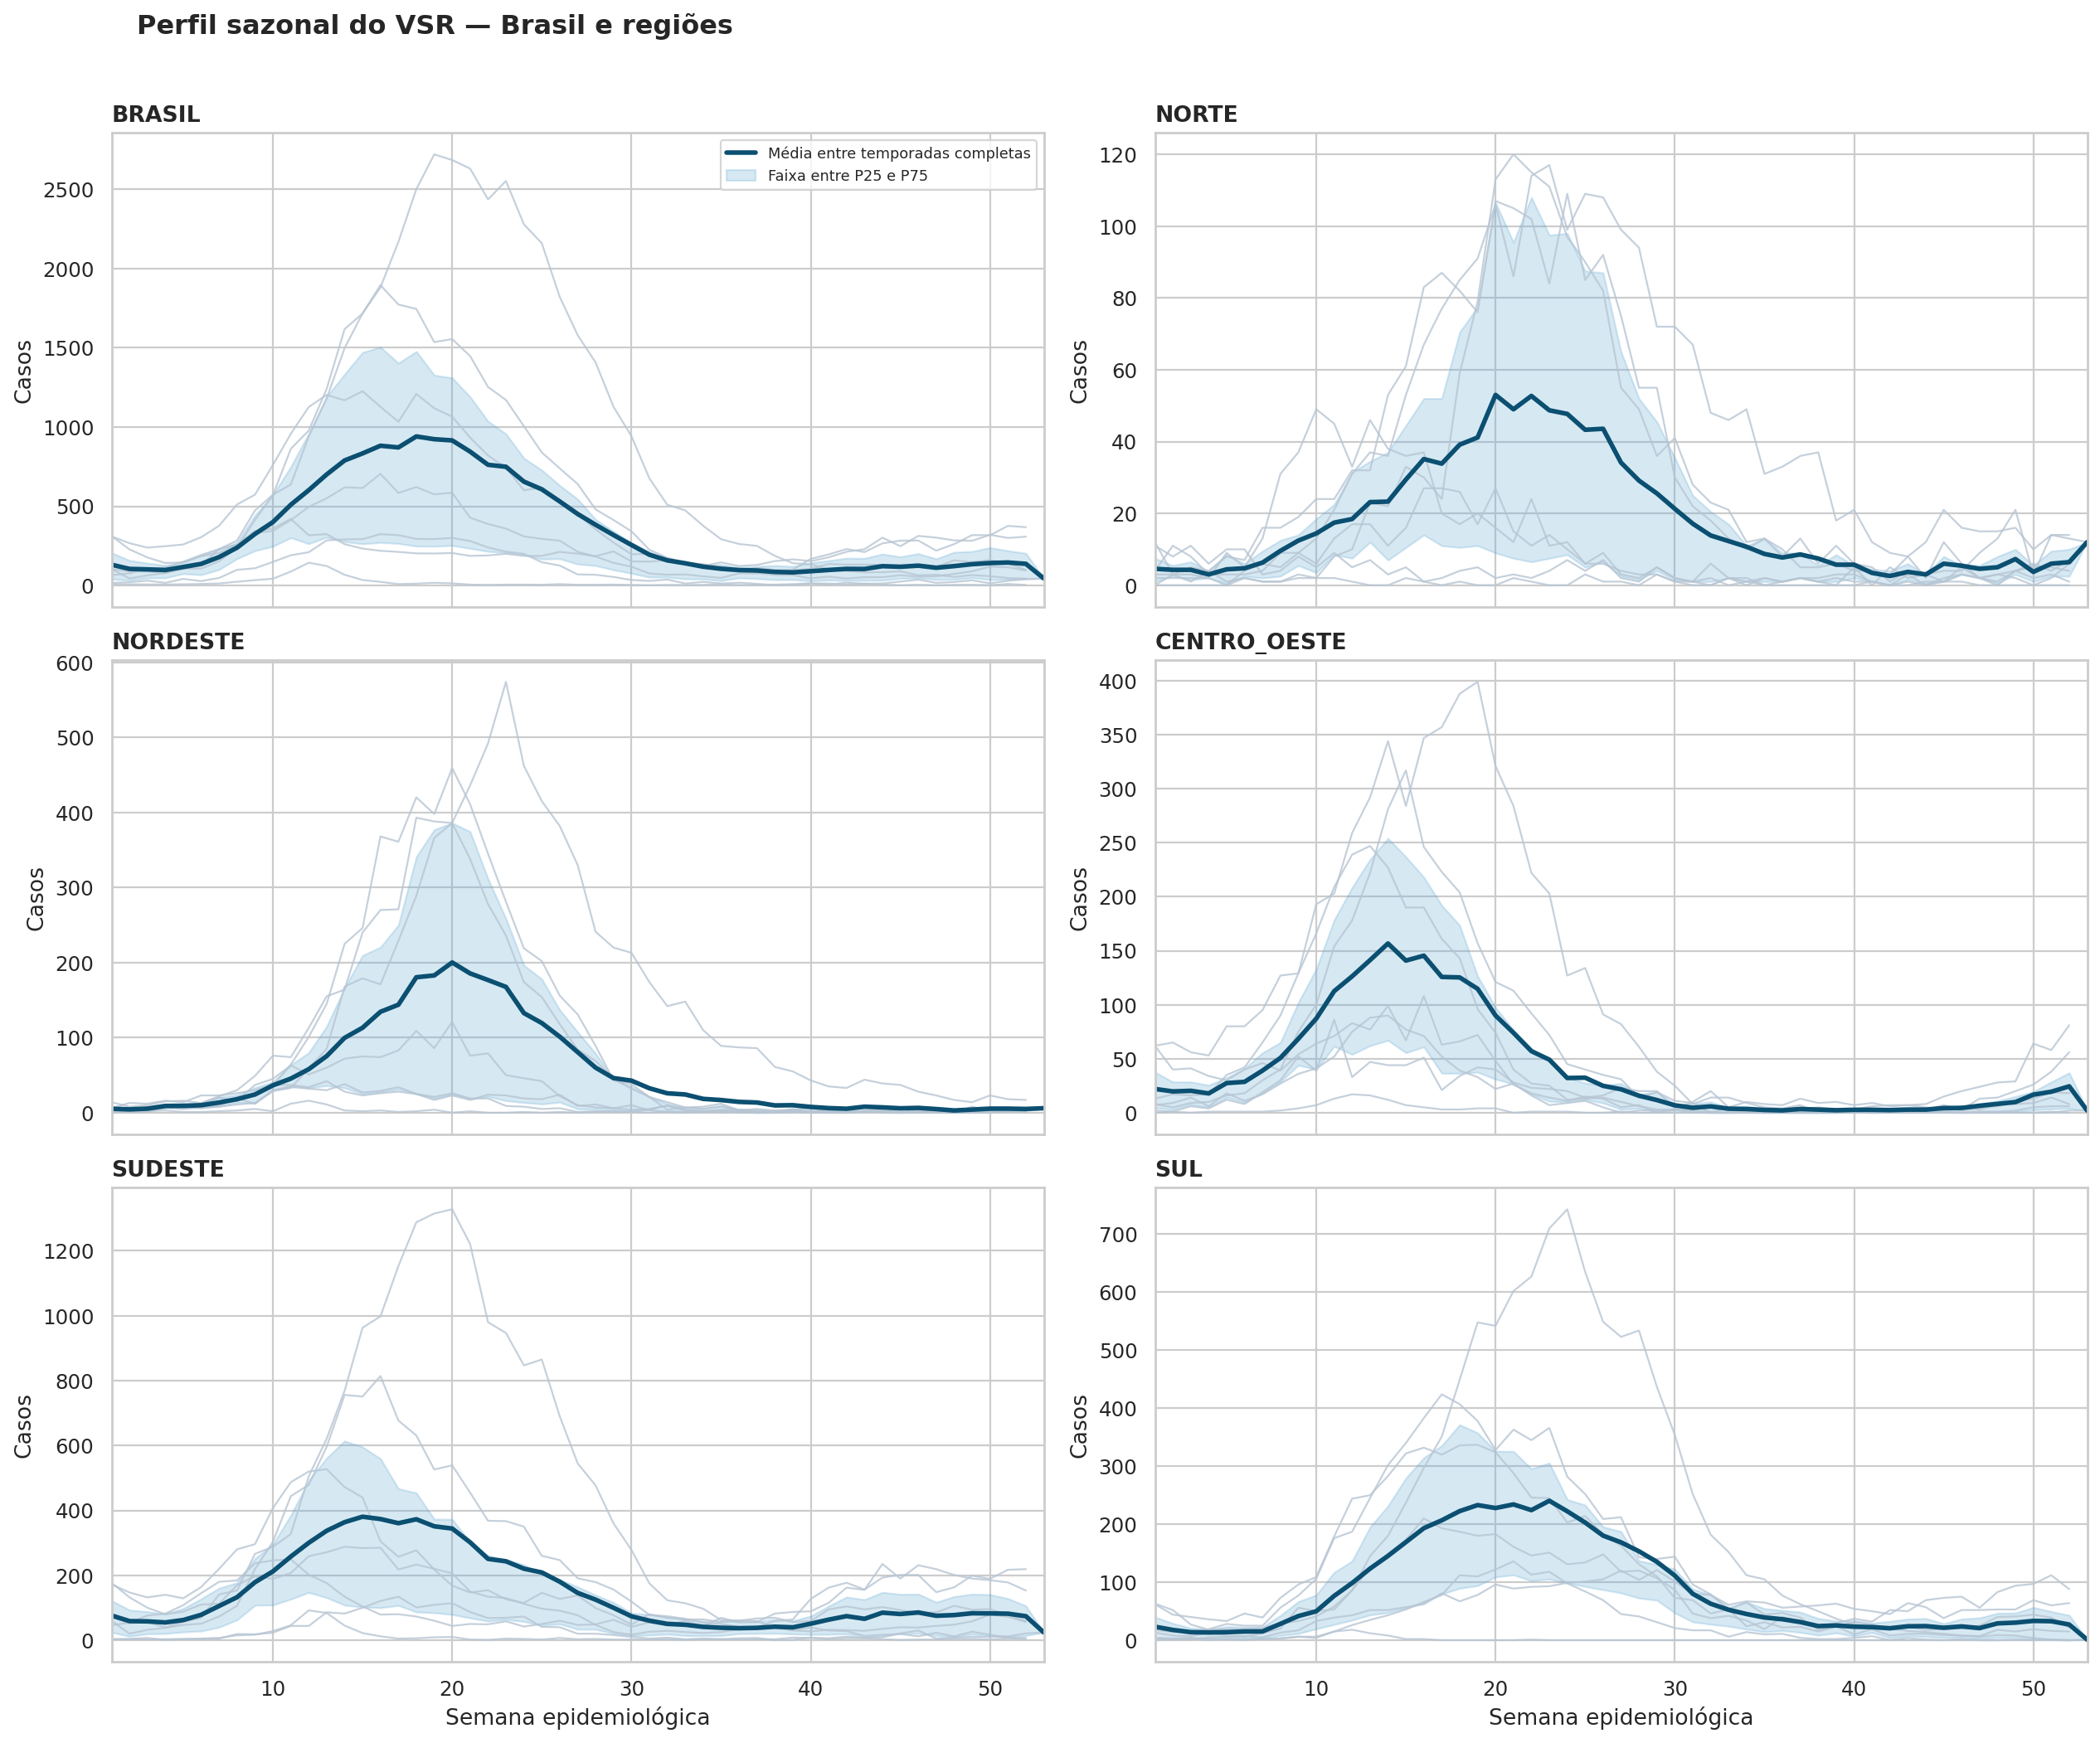
\includegraphics[width=\textwidth,height=.67\textheight,keepaspectratio]{sazonalidade_brasil_regioes.png}
    \end{column}
    \begin{column}{.40\textwidth}
      \begin{itemize}
        \item Picos nacionais apareceram aproximadamente entre as semanas epidemiológicas 11 e 19.
        \item Sudeste e Centro-Oeste tiveram padrão relativamente mais precoce e concentrado.
        \item O Nordeste mostrou picos mais tardios em anos recentes.
        \item Treze UFs têm mais de 50\% das semanas maduras sem casos registrados.
      \end{itemize}
      \vspace{.2cm}
      \small Brasil e regiões oferecem séries mais densas. UFs esparsas serão avaliadas com maior cautela.
    \end{column}
  \end{columns}
\end{frame}

\begin{frame}{Nível e variabilidade entre temporadas}
  \begin{columns}[T,onlytextwidth]
    \begin{column}{.58\textwidth}
      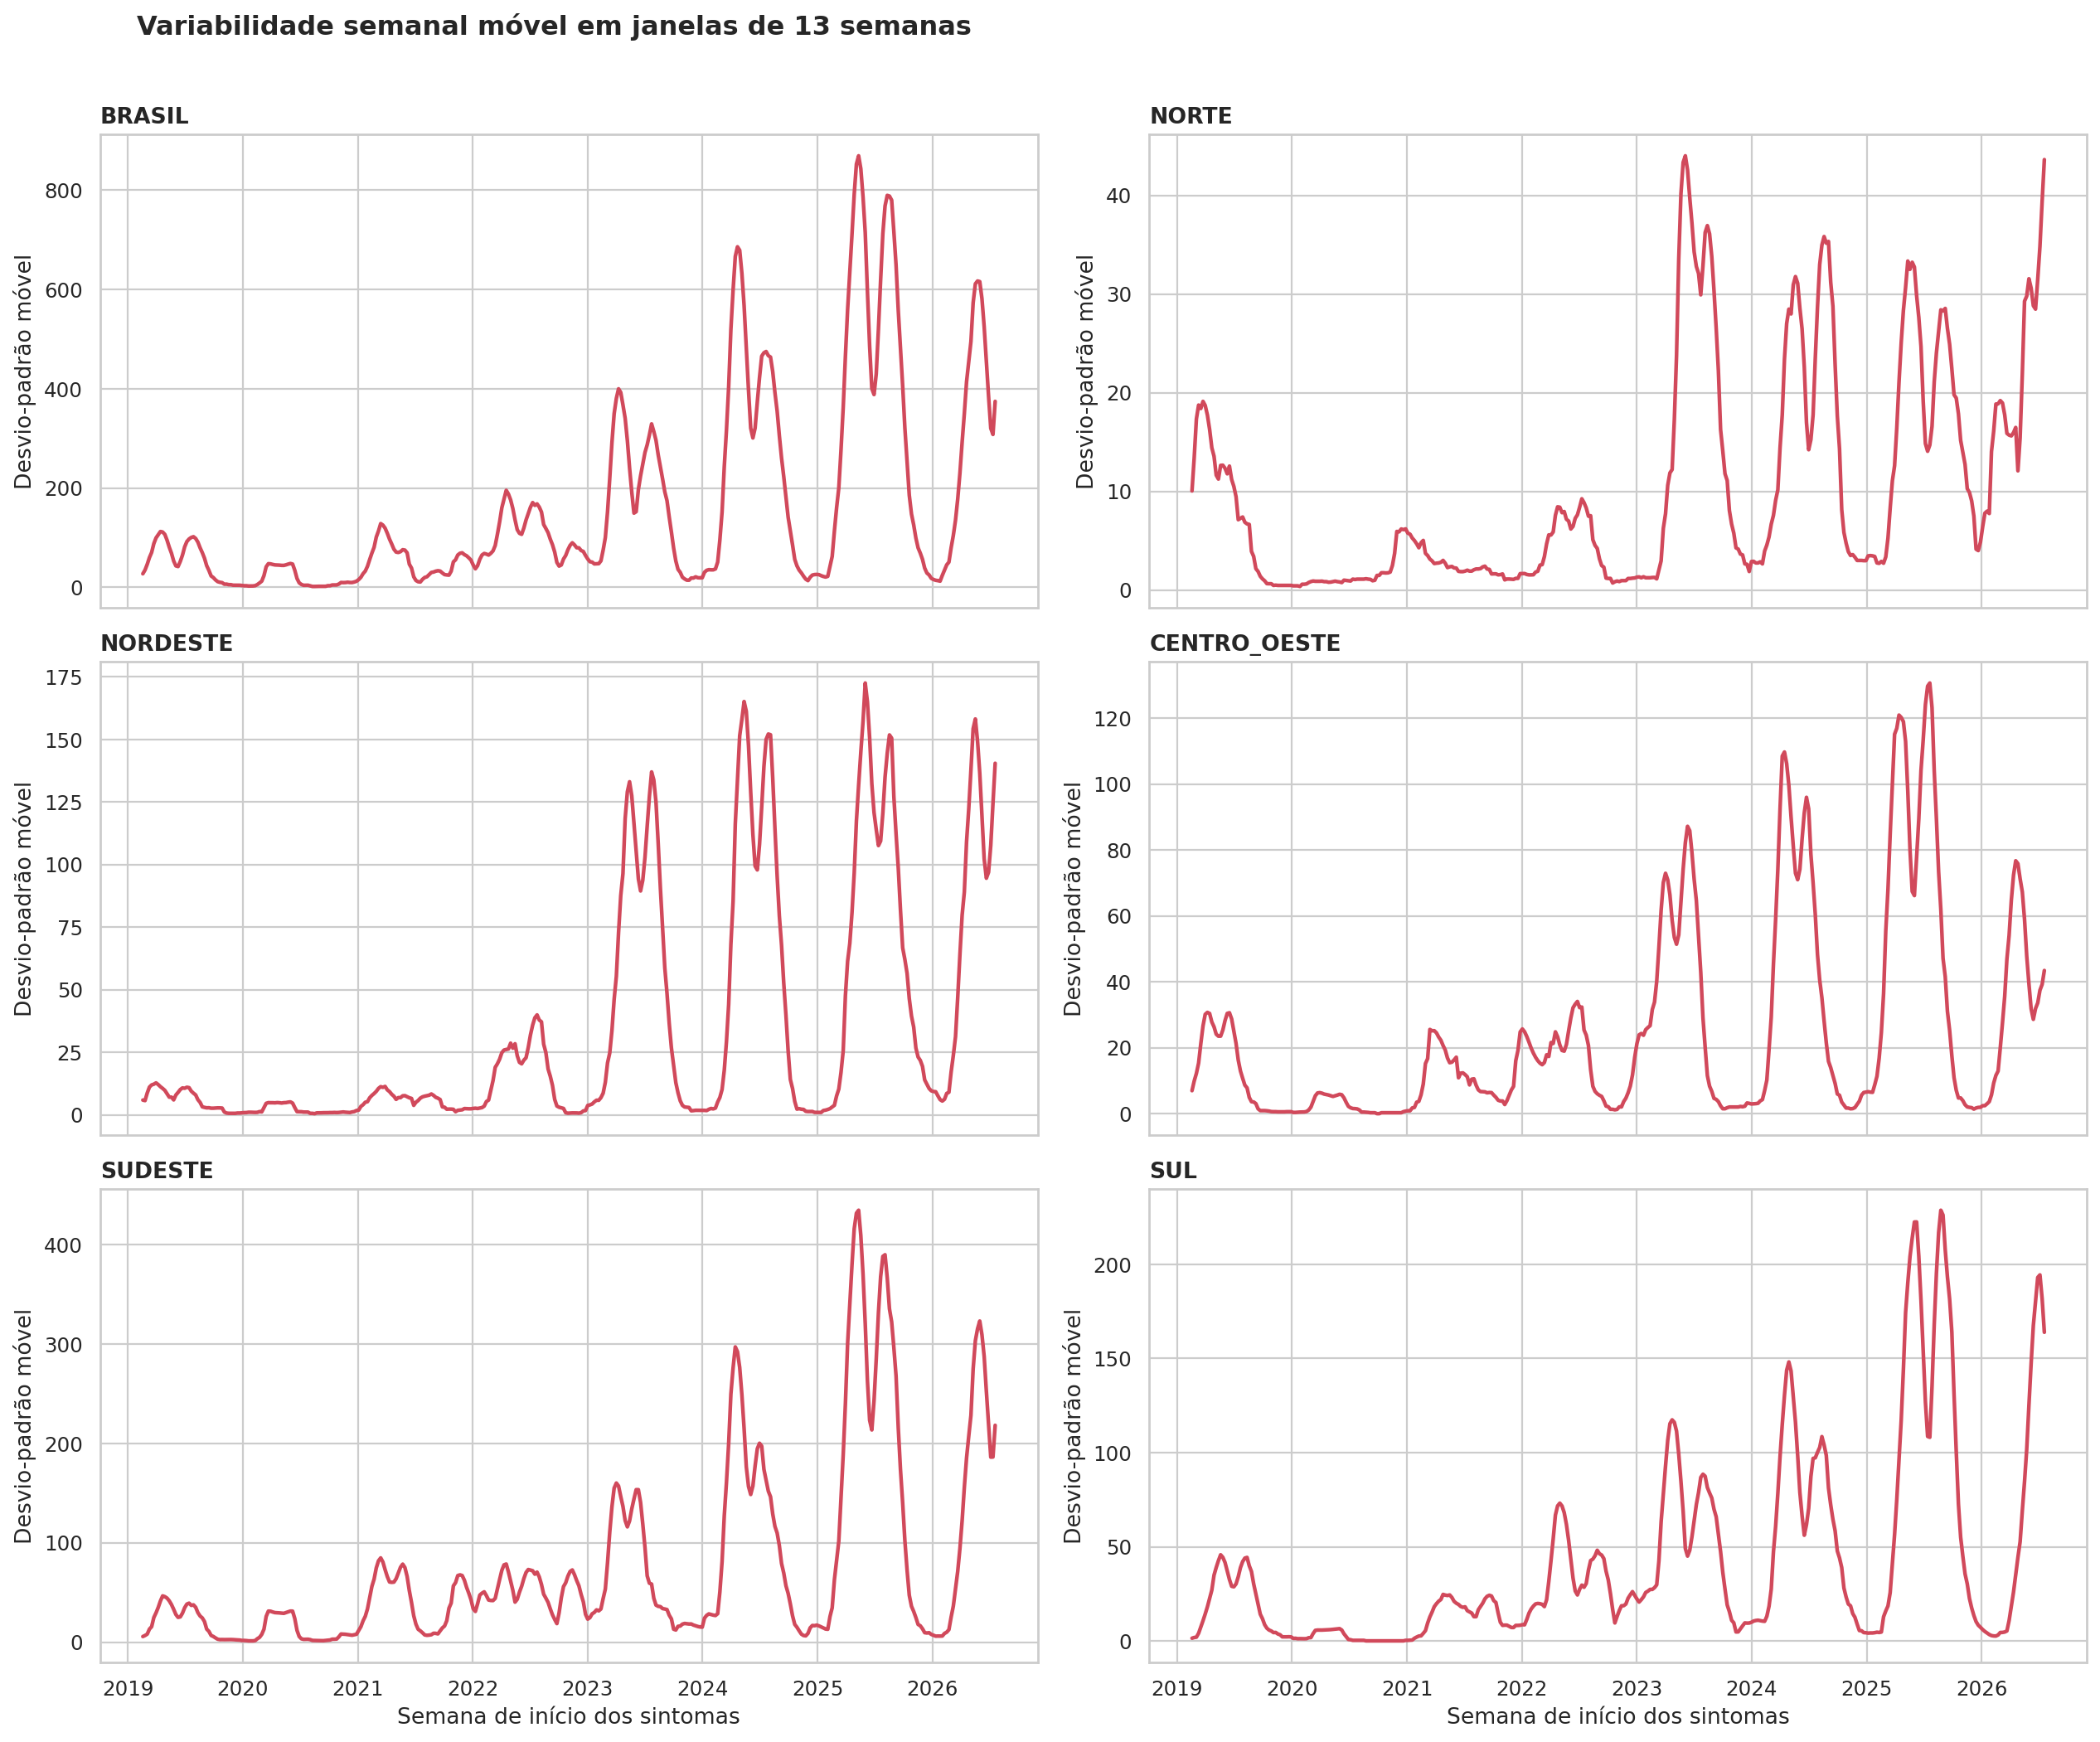
\includegraphics[width=\textwidth,height=.69\textheight,keepaspectratio]{variabilidade_movel_13s_brasil_regioes.png}
    \end{column}
    \begin{column}{.38\textwidth}
      \begin{itemize}
        \item Média semanal no Brasil: 287,9 em 2022 e 829,8 em 2025.
        \item Desvio-padrão semanal: 173,7 em 2022 e 912,3 em 2025.
        \item As temporadas recentes tiveram maior nível e maior oscilação.
      \end{itemize}
      \vspace{.2cm}
      \small O estudo descreve a mudança observada. Não atribuímos essa mudança a uma causa única.
    \end{column}
  \end{columns}
\end{frame}

\begin{frame}{Modelos candidatos e referência sazonal}
  \begin{block}{Referência obrigatória}
    \[
      \widehat{y}_{t+h} = y_{t+h-52}
    \]
    A previsão usa a semana epidemiológica equivalente da temporada anterior. Um modelo mais complexo precisa superá-la de modo consistente.
  \end{block}
  \vspace{.25cm}
  \begin{columns}[T,onlytextwidth]
    \begin{column}{.23\textwidth}\textcolor{pucblue}{\textbf{Ingênuo}}\\ \small Mantém o último valor observado.\end{column}
    \begin{column}{.23\textwidth}\textcolor{pucblue}{\textbf{ETS / Holt-Winters}}\\ \small Representa nível, tendência e sazonalidade.\end{column}
    \begin{column}{.23\textwidth}\textcolor{pucblue}{\textbf{SARIMA}}\\ \small Representa dependência temporal e ciclo sazonal.\end{column}
    \begin{column}{.23\textwidth}\textcolor{pucblue}{\textbf{Hierárquico}}\\ \small Busca coerência entre UF, região e Brasil.\end{column}
  \end{columns}
\end{frame}

\begin{frame}{Validação temporal e próximos passos}
  \begin{columns}[T,onlytextwidth]
    \begin{column}{.55\textwidth}
      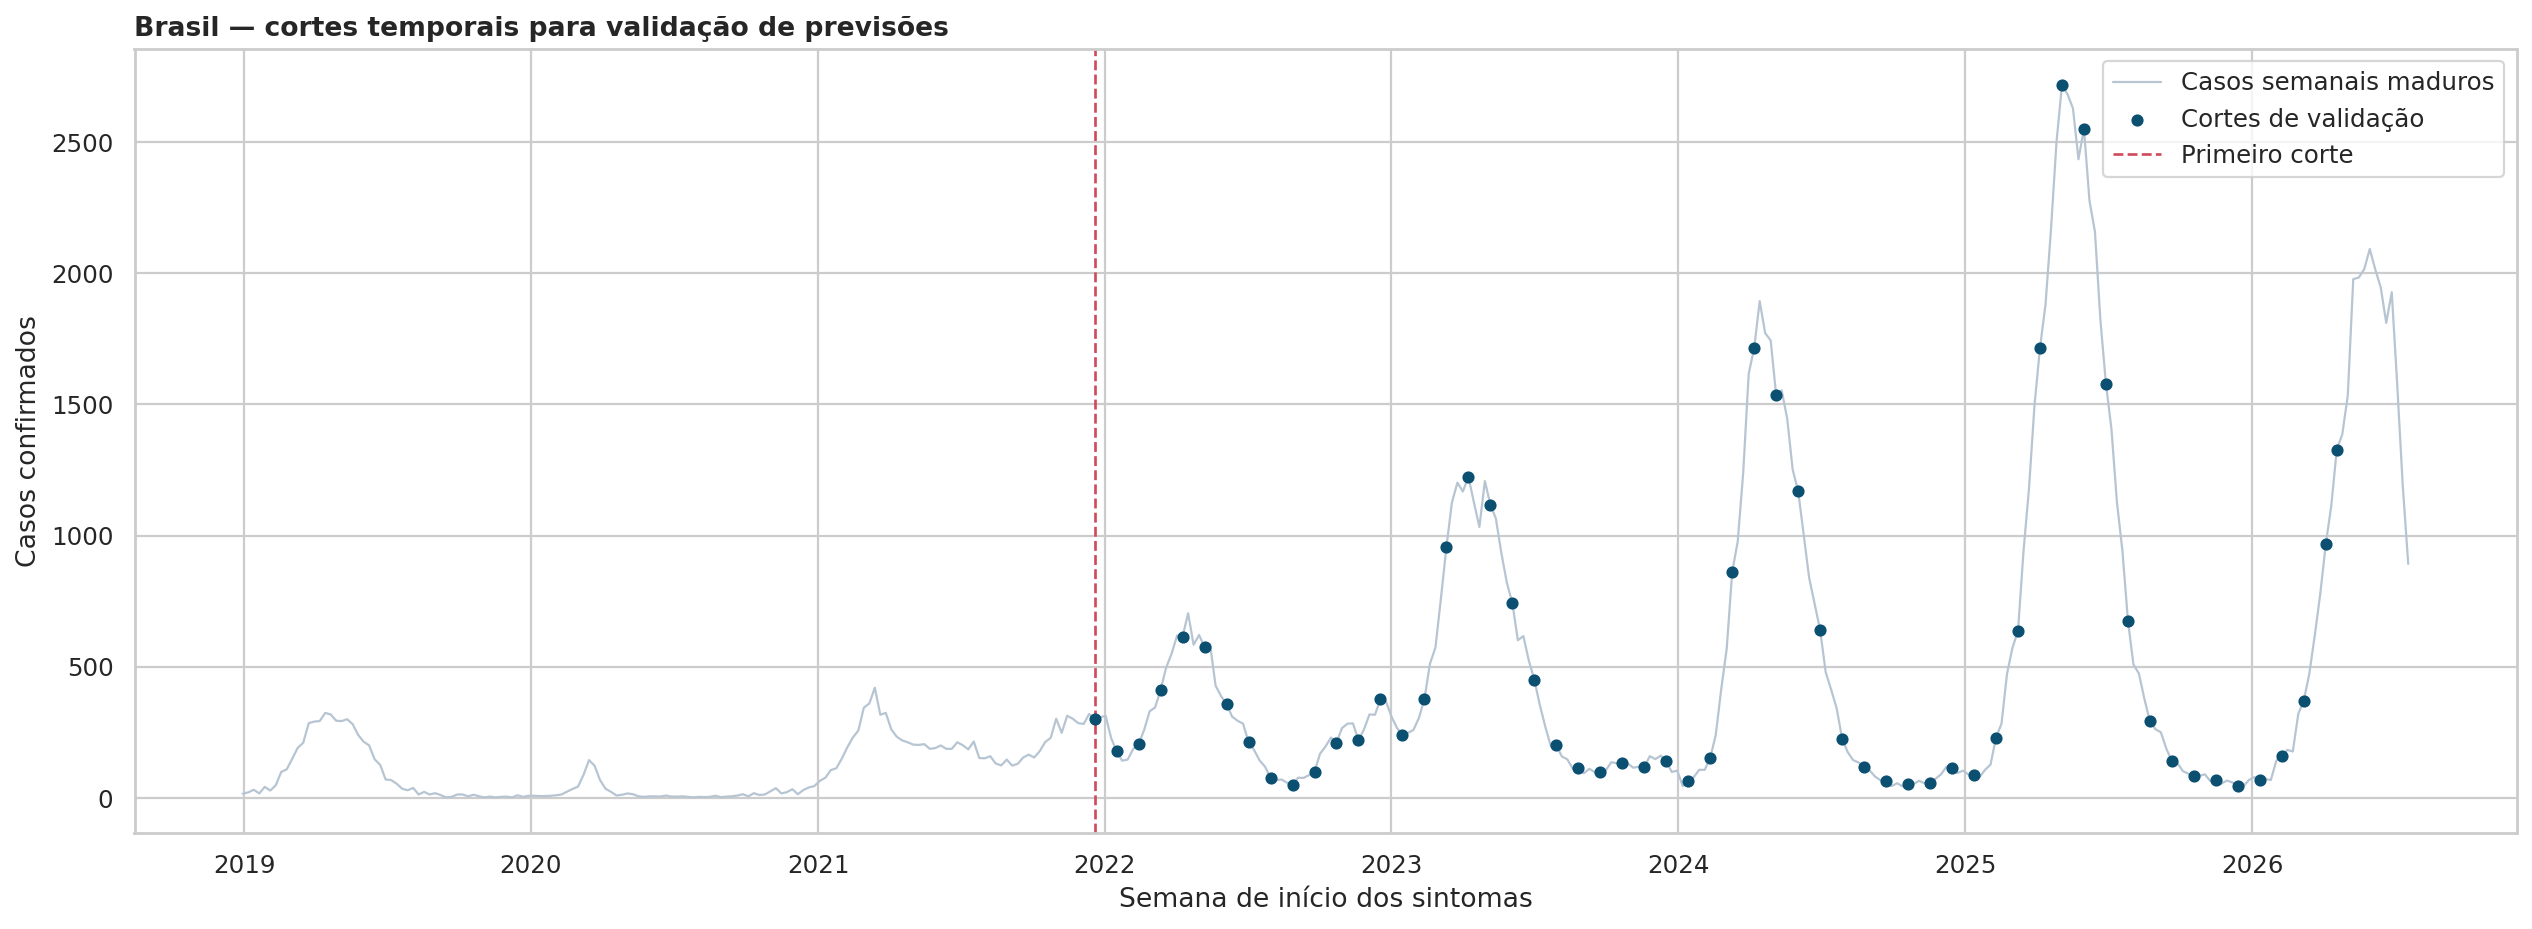
\includegraphics[width=\textwidth,height=.66\textheight,keepaspectratio]{calendario_validacao_brasil.png}
    \end{column}
    \begin{column}{.41\textwidth}
      \begin{itemize}
        \item 58 cortes temporais por série.
        \item Treino inicial de 156 semanas, aproximadamente três anos.
        \item Janela de treino expansiva.
        \item Horizontes de 1, 4, 8 e 13 semanas.
      \end{itemize}
      \vspace{.2cm}
      \small Avaliaremos MAE, RMSE e MASE. A próxima etapa compara cada candidato com a referência sazonal, sempre fora da amostra.
    \end{column}
  \end{columns}
\end{frame}

\end{document}
